\documentclass{article}




\usepackage{fullpage}
\usepackage{nopageno}
\usepackage{amsmath}
\usepackage{amsfonts}
\usepackage{graphicx}
\usepackage{framed}
\usepackage{algorithmic}
\usepackage{xcolor}

\definecolor{dark_red}{rgb}{0.5,0.0,0.0}
\definecolor{dark_green}{rgb}{0.0,0.5,0.0}
\definecolor{dark_blue}{rgb}{0.0,0.0,0.5}
\definecolor{blue}{rgb}{0.0,0.0,1.0}

\newcommand{\dr}[1]{\textcolor{dark_red}{#1}}
\newcommand{\dg}[1]{\textcolor{dark_green}{#1}}
\newcommand{\db}[1]{\textcolor{dark_blue}{#1}}
\newcommand{\blue}[1]{\textcolor{blue}{#1}}



\begin{document}

\section*{Repeating functions}


Let \(f(x)\) denote an arbitrary single variable function. Given an arbitrary nonnegative integer \(k\), the notation \(f^k(x)\) means to apply function \(f\) a total of \(k\) times to input value \(x\):

\[f^k(x) = \underbrace{f(f(...f(}_k x)...))\]

When \(k = 0\), \(f^0(x) = x\) which is the identity function that does not modify the input \(x\).


Moreover, if function \(f\) has an inverse \(f^{-1}\), then given an arbitrary nonnegative integer \(k\), the notation \(f^{-k}(x)\) means to apply the inverse function \(f^{-1}\) a total of \(k\) times to input value \(x\):

\[f^{-k}(x) = \underbrace{f^{-1}(f^{-1}(...f^{-1}(}_k x)...))\]

In general, when given an arbitrary integer \(k\), 

\[f^k(x) = \left\{\begin{array}{cc} \underbrace{f(f(...f(}_k x)...)) & (k > 0) \\ x & (k = 0) \\ \underbrace{f^{-1}(f^{-1}(...f^{-1}(}_{|k|} x)...)) & (k < 0) \end{array}\right.\]

More explicitly,

\begin{itemize}
\item ... 
\item \(f^{-4}(x) = f^{-1}(f^{-1}(f^{-1}(f^{-1}(x))))\)
\item \(f^{-3}(x) = f^{-1}(f^{-1}(f^{-1}(x)))\)
\item \(f^{-2}(x) = f^{-1}(f^{-1}(x))\)
\item \(f^{-1}(x) = f^{-1}(x)\)
\item \(f^0(x) = x\)
\item \(f^1(x) = f(x)\)
\item \(f^2(x) = f(f(x))\)
\item \(f^3(x) = f(f(f(x)))\)
\item \(f^4(x) = f(f(f(f(x))))\)
\item ... 
\end{itemize}

In addition, functions can also be ``partially" applied, provided that fractional applications are even possible. \(f^{1/2}\) is a function that when applied twice to \(x\) yields \(f(x)\):
\[f^{1/2}(f^{1/2}(x)) = f(x)\]


\vspace{5mm}

In many cases, repeatedly applying a function \(f\) to itself can be difficult. Consider for example the function \(f(x) = 3x - 10\). It is then the case that:  

\begin{itemize}
\item ...
\item \(f^{-4}(x) = f^{-1}(f^{-1}(f^{-1}(f^{-1}(x)))) = \frac{1}{81}x + \frac{400}{81}\)
\item \(f^{-3}(x) = f^{-1}(f^{-1}(f^{-1}(x))) = \frac{1}{27}x + \frac{130}{27}\)
\item \(f^{-2}(x) = f^{-1}(f^{-1}(x)) = \frac{1}{9}x + \frac{40}{9}\)
\item \(f^{-1}(x) = f^{-1}(x) = \frac{1}{3}x + \frac{10}{3}\)
\item \(f^0(x) = x\)
\item \(f^1(x) = f(x) = 3x - 10\)
\item \(f^2(x) = f(f(x)) = 9x - 40\) % = 3(3x - 10) - 10  
\item \(f^3(x) = f(f(f(x))) = 27x - 130\) % = 3(9x - 40) - 10
\item \(f^4(x) = f(f(f(f(x)))) = 81x - 400\) % = 3(27x - 130) - 10
\item ...
\item \(f^k(x) = \underbrace{f(f(...f(}_k x)...)) = ???\)
\item ...
\end{itemize}

\(f^k(x)\) becomes more complex as \(k\) gets large, and computing each successive \(f^k(x)\) becomes more and more challenging. Finding a general formula for \(f^k(x)\) is also challenging. However, it is possible to ``convert" \(f\) to a simpler function \(g\) that is easy to repeat. 

\vspace{5mm}

If \(f(x) = h(g(h^{-1}(x)))\), then since adjacent invocations of \(h\) and \(h^{-1}\) cancel out, 
\begin{itemize}
\item ... 
\item \(f^{-4}(x) = f^{-1}(f^{-1}(f^{-1}(f^{-1}(x)))) = h(g^{-4}(h^{-1}(x)))\)
\item \(f^{-3}(x) = f^{-1}(f^{-1}(f^{-1}(x))) = h(g^{-3}(h^{-1}(x)))\)
\item \(f^{-2}(x) = f^{-1}(f^{-1}(x)) = h(g^{-2}(h^{-1}(x)))\)
\item \(f^{-1}(x) = f^{-1}(x) = h(g^{-1}(h^{-1}(x)))\)
\item \(f^0(x) = x\)
\item \(f^1(x) = f(x) = h(g(h^{-1}(x)))\)
\item \(f^2(x) = f(f(x)) = h(g^2(h^{-1}(x)))\)
\item \(f^3(x) = f(f(f(x))) = h(g^3(h^{-1}(x)))\)
\item \(f^4(x) = f(f(f(f(x)))) = h(g^4(h^{-1}(x)))\)
\item ...
\item \(f^k(x) = \underbrace{f(f(...f(}_k x)...)) = h(g^k(h^{-1}(x)))\)
\item ...
\end{itemize}

For an arbitrary integer \(k\), 

\[f^k(x) = h(g^k(h^{-1}(x)))\]

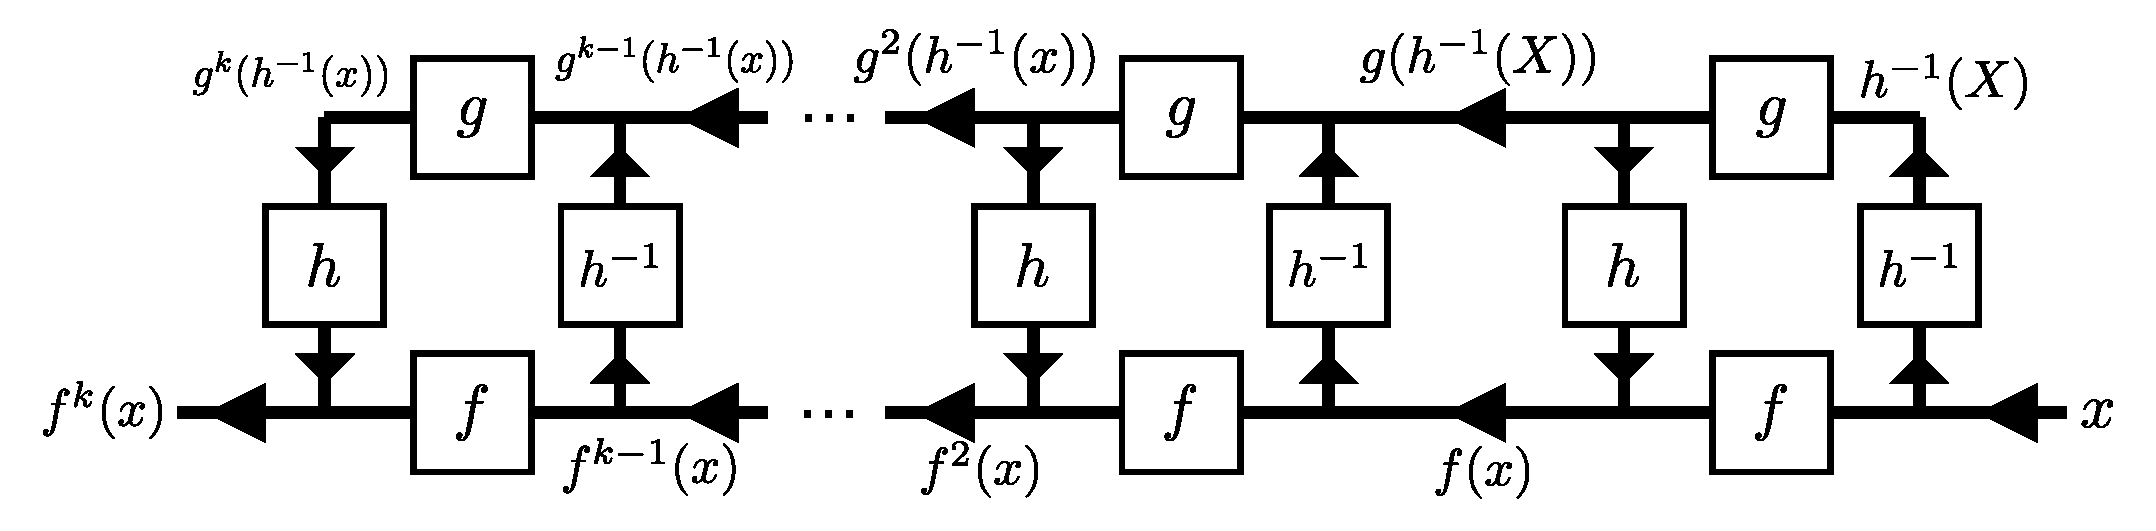
\includegraphics[width = \textwidth]{repeating_function}

\(f(x) = 3x - 10\) can be re-expressed as \(f(x) = 3x - 10 = 3(x - 5) + 5 = h(g(h^{-1}(x)))\) where \(g(x) = 3x\) and \(h(x) = x + 5\) so \(h^{-1}(x) = x - 5\).

Given an arbitrary nonnegative integer \(k\), \(g\) repeated \(k\) times is \(g^k(x) = 3^k x\). We can now derive a general expression for repeating \(f\) a total of \(k\) times:

\[f^k(x) = h(g^k(h^{-1}(x))) = 3^k(x - 5) + 5\]

This expression is also valid for negative values of \(k\) as well. Moreover, in this case \(k\) can take on fractional values as well.


\vspace{5mm}

As another example, let \(f(x) = x^2 - 8x + 20\). It is the case that \(f(x) = (x - 4)^2 + 4 = h(g(h^{-1}(x)))\) where \(g(x) = x^2\) and \(h(x) = x + 4\) so \(h^{-1}(x) = x - 4\).

Given an arbitrary nonnegative integer \(k\), \(g\) repeated \(k\) times is \(g^k(x) = x^{2^k}\). We can now derive a general expression for repeating \(f\) a total of \(k\) times:

\[f^k(x) = h(g^k(h^{-1}(x))) = (x - 4)^{2^k} + 4\]

This expression is also valid for negative values of \(k\) as well, provided that \(x \geq 4\) so the function is 1 to 1. Moreover, in this case \(k\) can take on fractional values as well.




\section*{Linear mappings and matrices}

Let \(A\) be an \(n \times n\) matrix. \(A\) is the coefficient matrix of a linear mapping \(L_A\) where the domain and codomain are both \(\mathbb{R}^n\). Given an arbitrary number \(k\), \(A^k\) is the coefficient matrix of \(L_A^k\). \(A^k\) is \(A\) multiplied by itself \(k\) times.

For example, let \(A = \begin{bmatrix} 1 & 4 \\ 2 & 3 \end{bmatrix}\). Multiplying \(A\) by itself gives:

\begin{itemize}
\item \(A^0 = I = \begin{bmatrix} 1 & 0 \\ 0 & 1 \end{bmatrix}\)
\item \(A^1 = A = \begin{bmatrix} 1 & 4 \\ 2 & 3 \end{bmatrix}\)
\item \(A^2 = A \cdot A = \begin{bmatrix} 9 & 16 \\ 8 & 17 \end{bmatrix}\) 
\item \(A^3 = A \cdot A \cdot A = \begin{bmatrix} 41 & 84 \\ 42 & 83 \end{bmatrix}\) 
\item \(A^4 = A \cdot A \cdot A \cdot A = \begin{bmatrix} 209 & 416 \\ 208 & 417 \end{bmatrix}\) 
\item ...
\item \(A^k = \underbrace{A \cdot A \cdot ... \cdot A}_k = ???\)
\item ...
\end{itemize}

\(A^k\) becomes more complex as \(k\) gets large, and computing each successive \(A^k\) becomes more and more challenging. Finding a general formula for \(A^k\) is also challenging. However, it is possible to ``convert" \(A\) to a simpler matrix \(\Lambda\) that is easy to repeat. 

In a similar manner to how the function \(f(x)\) was being re-expressed as \(f(x) = h(g(h^{-1}(x)))\) where \(g\) is easy to repeat, matrix \(A\) will be re-expressed as:
\[A = P \Lambda P^{-1}\]

In general, given two square matrices \(A\) and \(B\), if there exists an invertible matrix \(P\) such that \(A = PBP^{-1}\), then \(A\) and \(B\) are said to be {\bf similar}.

\(\Lambda\) will be a matrix that is easy to multiply by itself, and the easiest matrices to multiply by themselves are diagonal matrices. With regards to the linear mapping denoted by a diagonal matrix, each component of the input vector influences only the corresponding component of the output vector, and there is no ``cross talk" between the components. Given an arbitrary diagonal matrix:

\[\Lambda  = \begin{bmatrix} 
\lambda_1 & 0 & 0 & \cdots & 0 \\ 
0 & \lambda_2 & 0 & \cdots & 0 \\ 
0 & 0 & \lambda_3 & \cdots & 0 \\ 
\vdots & \vdots & \vdots & \ddots & \vdots \\
0 & 0 & 0 & \cdots & \lambda_n \end{bmatrix}\]

multiplying \(\Lambda\) by itself \(k\) times is clearly:

\[\Lambda^k  = \begin{bmatrix} 
\lambda_1^k & 0 & 0 & \cdots & 0 \\ 
0 & \lambda_2^k & 0 & \cdots & 0 \\ 
0 & 0 & \lambda_3^k & \cdots & 0 \\ 
\vdots & \vdots & \vdots & \ddots & \vdots \\
0 & 0 & 0 & \cdots & \lambda_n^k \end{bmatrix}\]

With \(A = P \Lambda P^{-1}\), it is then the case that \(A^k = P \Lambda^k P^{-1}\). When \(A\) is expressed in the form \(A = P \Lambda P^{-1}\) where \(\Lambda\) is a diagonal matrix, \(A\) is said to have been {\bf diagonalized} by matrix \(P\).

The question is now how to find matrices \(\Lambda\) and \(P\) given matrix \(A\). To address this problem, the concept of ``eigenvalues" and ``eigenvectors" will be introduced. 




\section*{Eigenvalues and Eigenvectors}

Given and \(n \times n\) matrix \(A\), we want an \(n \times n\) diagonal matrix \(\Lambda\) and an \(n \times n\) invertible matrix \(P\) such that \(A = P\Lambda P^{-1}\). Let \(\mathbf{p}_1\), \(\mathbf{p}_2\), ..., \(\mathbf{p}_n\) denote the columns of \(P\):

\[P = \begin{bmatrix} \mathbf{p}_1 & \mathbf{p}_2 & ... & \mathbf{p}_n \end{bmatrix}\]

Let \(\lambda_1\), \(\lambda_2\), ..., \(\lambda_n\) denote the diagonal entries of \(\Lambda\):

\[\Lambda = \begin{bmatrix} \lambda_1 & 0 & \cdots & 0 \\ 0 & \lambda_2 & \cdots & 0 \\ \vdots & \vdots & \ddots & \vdots \\ 0 & 0 & \cdots & \lambda_n \end{bmatrix}\] 

\(P\) denotes a linear mapping that takes a coefficient vector \(\begin{bmatrix} c_1 \\ c_2 \\ \vdots \\ c_n \end{bmatrix}\) and returns the linear combination of the columns of \(P\) using the coefficients:

\[P\begin{bmatrix} c_1 \\ c_2 \\ \vdots \\ c_n \end{bmatrix} = c_1\mathbf{p}_1 + c_2\mathbf{p}_2 + ... + c_n\mathbf{p}_n\]

In contrast, \(P^{-1}\) denotes a linear mapping that takes an arbitrary vector \(\mathbf{x}\) and returns the vector of coefficients \(\begin{bmatrix} c_1 \\ c_2 \\ \vdots \\ c_n \end{bmatrix}\) that would express \(\mathbf{x}\) as a linear combination of the columns of \(P\):

\[P^{-1}\mathbf{x} = \begin{bmatrix} c_1 \\ c_2 \\ \vdots \\ c_n \end{bmatrix} \quad\text{where}\quad c_1\mathbf{p}_1 + c_2\mathbf{p}_2 + ... + c_n\mathbf{p}_n = \mathbf{x}\]

Any vector \(\mathbf{x}\) can be denoted by either its own components or using the coefficients \(\begin{bmatrix} c_1 \\ c_2 \\ \vdots \\ c_n \end{bmatrix}\) where \(c_1\mathbf{p}_1 + c_2\mathbf{p}_2 + ... + c_n\mathbf{p}_n = \mathbf{x}\). 

\begin{align*}
A\mathbf{x} = & P\Lambda P^{-1}\mathbf{x} = P\Lambda\begin{bmatrix} c_1 \\ c_2 \\ \vdots \\ c_n \end{bmatrix} = P\begin{bmatrix} \lambda_1 c_1 \\ \lambda_2 c_2 \\ \vdots \\ \lambda_n c_n \end{bmatrix} = (\lambda_1 c_1)\mathbf{p}_1 + (\lambda_2 c_2)\mathbf{p}_2 + ... + (\lambda_n c_n)\mathbf{p}_n
\end{align*}
so multiplication by matrix \(A\) increases each coefficient \(c_i\) by a factor of \(\lambda_i\). If \(\mathbf{x} = \mathbf{p}_i\), then \(A\mathbf{x} = \lambda_i \mathbf{p}_i\), so the \(i^{\text{th}}\) column of \(P\) has the property that \(A\mathbf{p}_i = \lambda_i \mathbf{p}_i\).

Any nonzero vector that changes by a scalar multiple when multiplied by matrix \(A\) is called an {\bf eigenvector} of \(A\), and the corresponding scalar is an {\bf eigenvalue} of \(A\). For \(\lambda\) to be an eigenvalue of \(A\), the equation \(A\mathbf{p} = \lambda\mathbf{p}\) must have nontrivial solutions for \(\mathbf{p}\). \(A\mathbf{p} = \lambda\mathbf{p} \iff (A - \lambda I)\mathbf{p} = \mathbf{0}\) so the matrix \(A - \lambda I\) must have a nontrivial null space and be singular (noninvertible). A straightforwards algebraic condition for \(A - \lambda I\) to be noninvertible is for the determinant of \(A - \lambda I\) to be \(0\):

\[\text{det}(A - \lambda I) = 0\]

\(\text{det}(A - \lambda I)\) is a degree \(n\) polynomial with respect to \(\lambda\). The polynomial \(\text{det}(A - \lambda I)\) is referred to as the {\bf characteristic polynomial} of \(A\), and the equation \(\text{det}(A - \lambda I) = 0\) is referred to as the {\bf characteristic equation} of \(A\). All solutions to the characteristic equation are eigenvalues of \(A\). 

For each eigenvalue \(\lambda\), the null space of \(A - \lambda I\) is the {\bf eigenspace} of \(\lambda\), and all nonzero vectors from this null space are eigenvectors that correspond to eigenvalue \(\lambda\). The null space of \(A - \lambda I\) will always be nontrivial and contain nonzero vectors. 

According to the fundamental theorem of algebra, the characteristic polynomial has the factorization:
\[\text{det}(A - \lambda I) = (-1)^n(\lambda - c_1)^{m_1}(\lambda - c_2)^{m_2} \cdots (\lambda - c_k)^{m_k}\]
where \(m_1 + m_2 + ... + m_k = n\).

For each \(i = 1, 2, ..., k\), with respect to the eigenvalue \(\lambda = c_i\), the exponent \(m_i\) is the {\bf multiplicity} of the eigenvalue \(c_i\). The eigenspace that corresponds to eigenvalue \(c_i\) will have between \(1\) and \(m_i\) dimensions. For matrix \(A\) to be fully diagonalizable, the dimension of each eigenspace must be at its maximum. 

To diagonalize \(A\), the diagonal entries of \(\Lambda\) are the eigenvalues of \(A\). Eigenvalues are repeated according to their multiplicity in the characteristic polynomial. For each eigenvalue \(\lambda_i\), a corresponding eigenvector \(\mathbf{p}_i\) is chosen. When there are multiple copies of the same eigenvalue, the chosen eigenvectors must be linearly independent. This is why the dimension of each eigenspace needs to match the multiplicity of the corresponding eigenvalue. The eigenvalues form the diagonal entries of \(\Lambda\), and the chosen eigenvectors form the columns of \(P\). It is important to order the columns of \(P\) so the the \(i^{\text{th}}\) column is an eigenvector of the \(i^{\text{th}}\) diagonal entry of \(\Lambda\). 
  
\[A = \begin{bmatrix} \mathbf{p}_1 & \mathbf{p}_2 & ... & \mathbf{p}_n \end{bmatrix}\begin{bmatrix} \lambda_1 & 0 & \cdots & 0 \\ 0 & \lambda_2 & \cdots & 0 \\ \vdots & \vdots & \ddots & \vdots \\ 0 & 0 & \cdots & \lambda_n \end{bmatrix}\begin{bmatrix} \mathbf{p}_1 & \mathbf{p}_2 & ... & \mathbf{p}_n \end{bmatrix}^{-1}\]

and for any \(k\), 

\[A^k = \begin{bmatrix} \mathbf{p}_1 & \mathbf{p}_2 & ... & \mathbf{p}_n \end{bmatrix}\begin{bmatrix} \lambda_1^k & 0 & \cdots & 0 \\ 0 & \lambda_2^k & \cdots & 0 \\ \vdots & \vdots & \ddots & \vdots \\ 0 & 0 & \cdots & \lambda_n^k \end{bmatrix}\begin{bmatrix} \mathbf{p}_1 & \mathbf{p}_2 & ... & \mathbf{p}_n \end{bmatrix}^{-1}\]


\vspace{5mm}

From the characteristic polynomial \(\text{det}(A - \lambda I) = (-1)^n(\lambda - c_1)^{m_1}(\lambda - c_2)^{m_2} \cdots (\lambda - c_k)^{m_k}\), when \(\lambda\) is set to \(0\), this equation becomes:

\begin{align*}
\text{det}(A) 
= & \text{det}(A - 0I) 
= (-1)^n(0 - c_1)^{m_1}(0 - c_2)^{m_2} \cdots (0 - c_k)^{m_k} \\
= & (-1)^n(-c_1)^{m_1}(-c_2)^{m_2} \cdots (-c_k)^{m_k} \\
= & (-1)^n(-1)^{m_1 + m_2 + ... + m_k}c_1^{m_1} c_2^{m_2} \cdots c_k^{m_k} \\
= & c_1^{m_1} c_2^{m_2} \cdots c_k^{m_k}
\end{align*}

The determinant of \(A\) can be easily computed if the eigenvalues and their respective multiplicities are known: \(\text{det}(A) = c_1^{m_1} c_2^{m_2} \cdots c_k^{m_k}\).  

\vspace{5mm}


\textbf{Examples:}
\begin{itemize}
%%%%%%%%%%%%%%%%%%%%%%%%%%%
\item Let \(A = \begin{bmatrix} 1 & 4 \\ 2 & 3 \end{bmatrix}\). The characteristic polynomial is:
\begin{align*}
\text{det}(A - \lambda I) = & \begin{vmatrix}
1 - \lambda & 4 \\ 
2 & 3 - \lambda 
\end{vmatrix} = (1 - \lambda)(3 - \lambda) - (2)(4) = (\lambda^2 - 4\lambda + 3) - 8 \\
= & \lambda^2 - 4\lambda - 5 = (\lambda + 1)(\lambda - 5)
\end{align*}
The eigenvalues are \(\lambda_1 = -1\) and \(\lambda_2 = 5\). \\
With respect to \(\lambda_1 = -1\) row reduction of \(A - \lambda_1 I\) proceeds as follows: 
\begin{align*}
A - (-1) I = 
\begin{bmatrix} 
2 & 4 \\ 
2 & 4 
\end{bmatrix} 
\xrightarrow{\begin{array}{c} R_2 \rightarrow R_2 - R_1 \end{array}} 
\begin{bmatrix} 
2 & 4 \\ 
0 & 0 
\end{bmatrix} 
\xrightarrow{\begin{array}{c} R_1 \rightarrow (1/2)R_1 \end{array}} 
\begin{bmatrix} 
1 & 2 \\ 
0 & 0 
\end{bmatrix} 
\end{align*} 
The eigenspace is \(\text{span}\left\{\begin{bmatrix} -2 \\ 1 \end{bmatrix}\right\}\) so let \(\mathbf{p}_1 = \begin{bmatrix} -2 \\ 1 \end{bmatrix}\). \\
With respect to \(\lambda_2 = 5\) row reduction of \(A - \lambda_2 I\) proceeds as follows: 
\begin{align*}
A - 5I = 
\begin{bmatrix} 
-4 & 4 \\ 
2 & -2 
\end{bmatrix} 
\xrightarrow{\begin{array}{c} R_2 \rightarrow R_2 + (1/2)R_1 \end{array}} 
\begin{bmatrix} 
-4 & 4 \\ 
0 & 0 
\end{bmatrix} 
\xrightarrow{\begin{array}{c} R_1 \rightarrow -(1/4)R_1 \end{array}} 
\begin{bmatrix} 
1 & -1 \\ 
0 & 0 
\end{bmatrix} 
\end{align*} 
The eigenspace is \(\text{span}\left\{\begin{bmatrix} 1 \\ 1 \end{bmatrix}\right\}\) so let \(\mathbf{p}_2 = \begin{bmatrix} 1 \\ 1 \end{bmatrix}\). \\
We now have \(\Lambda = \begin{bmatrix} \lambda_1 & 0 \\ 0 & \lambda_2 \end{bmatrix} = \begin{bmatrix} -1 & 0 \\ 0 & 5 \end{bmatrix}\) and \(P = \begin{bmatrix} \mathbf{p}_1 & \mathbf{p}_2 \end{bmatrix} = \begin{bmatrix} -2 & 1 \\ 1 & 1 \end{bmatrix}\). Computing \(P^{-1}\) gives:
\begin{align*}
& \left[\begin{array}{cc|cc}  
-2 & 1 & 1 & 0 \\ 
 1 & 1 & 0 & 1 
\end{array}\right] 
\xrightarrow{\begin{array}{c} R_1 \rightarrow -(1/2)R_1 \end{array}} 
\left[\begin{array}{cc|cc}  
1 & -1/2 & -1/2 & 0 \\ 
1 &      1 &     0 & 1 
\end{array}\right] \\
& \xrightarrow{\begin{array}{c} R_2 \rightarrow R_2 - R_1 \end{array}} 
\left[\begin{array}{cc|cc}  
1 & -1/2 & -1/2 & 0 \\ 
0 &  3/2 &   1/2 & 1 
\end{array}\right] 
\xrightarrow{\begin{array}{c} R_2 \rightarrow (2/3)R_2 \end{array}} 
\left[\begin{array}{cc|cc}  
1 & -1/2 & -1/2 &    0 \\ 
0 &     1 &   1/3 & 2/3 
\end{array}\right] \\ 
& \xrightarrow{\begin{array}{c} R_1 \rightarrow R_1 + (1/2)R_2 \end{array}} 
\left[\begin{array}{cc|cc}  
1 & 0 & -1/3 & 1/3 \\ 
0 & 1 &   1/3 & 2/3 
\end{array}\right]
\end{align*}
\(P^{-1} = \begin{bmatrix} -1/3 & 1/3 \\ 1/3 & 2/3 \end{bmatrix}\) so therefore:
\[A = \begin{bmatrix} -2 & 1 \\ 1 & 1 \end{bmatrix}\begin{bmatrix} -1 & 0 \\ 0 & 5 \end{bmatrix}\begin{bmatrix} -1/3 & 1/3 \\ 1/3 & 2/3 \end{bmatrix}\]  
%%%%%%%%%%%%%%%%%%%%%%%%%%%
\item Let \(A = \begin{bmatrix} 2 & 0 & 0 \\ -9 & -1 & 0 \\ -22 & -8 & 1 \end{bmatrix}\). The characteristic polynomial is:
\begin{align*}
\text{det}(A - \lambda I) = & \begin{vmatrix}
2 - \lambda & 0 & 0 \\ 
-9 & -1 - \lambda & 0 \\ 
-22 & -8 & 1 - \lambda
\end{vmatrix} = (2 - \lambda)(-1 - \lambda)(1 - \lambda)
\end{align*}
The eigenvalues are \(\lambda_1 = -1\), \(\lambda_2 = 1\), and \(\lambda_3 = 2\). \\
With respect to \(\lambda_1 = -1\), row reduction of \(A - \lambda_1 I\) yields: 
\[\begin{bmatrix} 
1 & 0 & 0 \\ 
0 & 1 & -1/4 \\
0 & 0 & 0 
\end{bmatrix}\]
The eigenspace is \(\text{span}\left\{\begin{bmatrix} 0 \\ 1/4 \\ 1 \end{bmatrix}\right\}\) so let \(\mathbf{p}_1 = \begin{bmatrix} 0 \\ 1/4 \\ 1 \end{bmatrix}\). \\
With respect to \(\lambda_2 = 1\), row reduction of \(A - \lambda_2 I\) yields: 
\[\begin{bmatrix} 
1 & 0 & 0 \\ 
0 & 1 & 0 \\
0 & 0 & 0 
\end{bmatrix}\]
The eigenspace is \(\text{span}\left\{\begin{bmatrix} 0 \\ 0 \\ 1 \end{bmatrix}\right\}\) so let \(\mathbf{p}_2 = \begin{bmatrix} 0 \\ 0 \\ 1 \end{bmatrix}\). \\
With respect to \(\lambda_3 = 2\), row reduction of \(A - \lambda_3 I\) yields: 
\[\begin{bmatrix} 
1 & 0 & -1/2 \\ 
0 & 1 & 3/2 \\
0 & 0 & 0 
\end{bmatrix}\]
The eigenspace is \(\text{span}\left\{\begin{bmatrix} 1/2 \\ -3/2 \\ 1 \end{bmatrix}\right\}\) so let \(\mathbf{p}_3 = \begin{bmatrix} 1/2 \\ -3/2 \\ 1 \end{bmatrix}\). \\
We now have \(\Lambda = \begin{bmatrix} \lambda_1 & 0 & 0 \\ 0 & \lambda_2 & 0 \\ 0 & 0 & \lambda_3 \end{bmatrix} = \begin{bmatrix} -1 & 0 & 0 \\ 0 & 1 & 0 \\ 0 & 0 & 2 \end{bmatrix}\) and \(P = \begin{bmatrix} \mathbf{p}_1 & \mathbf{p}_2 & \mathbf{p}_3 \end{bmatrix} = \begin{bmatrix} 0 & 0 & 1/2 \\ 1/4 & 0 & -3/2 \\ 1 & 1 & 1 \end{bmatrix}\). Computing \(P^{-1}\) gives \(P^{-1} = \begin{bmatrix} 12 & 4 & 0 \\ -14 & -4 & 1 \\ 2 & 0 & 0 \end{bmatrix}\) so therefore:
\[A = \begin{bmatrix} 0 & 0 & 1/2 \\ 1/4 & 0 & -3/2 \\ 1 & 1 & 1 \end{bmatrix}\begin{bmatrix} -1 & 0 & 0 \\ 0 & 1 & 0 \\ 0 & 0 & 2 \end{bmatrix}\begin{bmatrix} 12 & 4 & 0 \\ -14 & -4 & 1 \\ 2 & 0 & 0 \end{bmatrix}\]
%%%%%%%%%%%%%%%%%%%%%%%%%%%
\item Let \(A = \begin{bmatrix} -3 & 0 & 0 \\ 4 & 1 & 0 \\ -8 & 0 & 1 \end{bmatrix}\). The characteristic polynomial is:
\begin{align*}
\text{det}(A - \lambda I) = & \begin{vmatrix}
-3 - \lambda & 0 & 0 \\ 
4 & 1 - \lambda & 0 \\ 
-8 & 0 & 1 - \lambda
\end{vmatrix} = (-3 - \lambda)(1 - \lambda)^2
\end{align*}
The eigenvalues are \(\lambda_1 = -3\), and \(\lambda_2 = \lambda_3 = 1\). The eigenvalue of \(1\) has a multiplicity of \(2\). \\
With respect to \(\lambda_1 = -3\), row reduction of \(A - \lambda_1 I\) yields: 
\[\begin{bmatrix} 
1 & 0 & -1/2 \\ 
0 & 1 & 1/2 \\
0 & 0 & 0 
\end{bmatrix}\]
The eigenspace is \(\text{span}\left\{\begin{bmatrix} 1/2 \\ -1/2 \\ 1 \end{bmatrix}\right\}\) so let \(\mathbf{p}_1 = \begin{bmatrix} 1/2 \\ -1/2 \\ 1 \end{bmatrix}\). \\
With respect to \(\lambda_2 = \lambda_3 = 1\), row reduction of \(A - \lambda_2 I\) yields: 
\[\begin{bmatrix} 
1 & 0 & 0 \\ 
0 & 0 & 0 \\
0 & 0 & 0 
\end{bmatrix}\]
The eigenspace is \(\text{span}\left\{\begin{bmatrix} 0 \\ 1 \\ 0 \end{bmatrix}, \begin{bmatrix} 0 \\ 0 \\ 1 \end{bmatrix}\right\}\) so let \(\mathbf{p}_2 = \begin{bmatrix} 0 \\ 1 \\ 0 \end{bmatrix}\) and \(\mathbf{p}_3 = \begin{bmatrix} 0 \\ 0 \\ 1 \end{bmatrix}\). \\ 
We now have \(\Lambda = \begin{bmatrix} \lambda_1 & 0 & 0 \\ 0 & \lambda_2 & 0 \\ 0 & 0 & \lambda_3 \end{bmatrix} = \begin{bmatrix} -3 & 0 & 0 \\ 0 & 1 & 0 \\ 0 & 0 & 1 \end{bmatrix}\) and \(P = \begin{bmatrix} \mathbf{p}_1 & \mathbf{p}_2 & \mathbf{p}_3 \end{bmatrix} = \begin{bmatrix} 1/2 & 0 & 0 \\ -1/2 & 1 & 0 \\ 1 & 0 & 1 \end{bmatrix}\). Computing \(P^{-1}\) gives \(P^{-1} = \begin{bmatrix} 2 & 0 & 0 \\ 1 & 1 & 0 \\ -2 & 0 & 1 \end{bmatrix}\) so therefore: 
\[A = \begin{bmatrix} 1/2 & 0 & 0 \\ -1/2 & 1 & 0 \\ 1 & 0 & 1 \end{bmatrix}\begin{bmatrix} -3 & 0 & 0 \\ 0 & 1 & 0 \\ 0 & 0 & 1 \end{bmatrix}\begin{bmatrix} 2 & 0 & 0 \\ 1 & 1 & 0 \\ -2 & 0 & 1 \end{bmatrix}\]
%%%%%%%%%%%%%%%%%%%%%%%%%%%
\item Let \(A = \begin{bmatrix} -2 & 0 & 0 \\ 1 & 0 & 1 \\ 8 & -9 & 6 \end{bmatrix}\). The characteristic polynomial is:
\begin{align*}
\text{det}(A - \lambda I) = & \begin{vmatrix}
-2 - \lambda & 0 & 0 \\ 
1 & -\lambda & 1 \\ 
8 & -9 & 6 - \lambda
\end{vmatrix} = (-2 - \lambda)\begin{vmatrix}
-\lambda & 1 \\ 
-9 & 6 - \lambda
\end{vmatrix} = (-2 - \lambda)((-\lambda)(6 - \lambda) - (-9)(1)) \\
= & (-2 - \lambda)(\lambda^2 - 6\lambda + 9) 
= (-2 - \lambda)(3 - \lambda)^2
\end{align*}
The eigenvalues are \(\lambda_1 = -2\), and \(\lambda_2 = \lambda_3 = 3\). The eigenvalue of \(3\) has a multiplicity of \(2\). \\ 
With respect to \(\lambda_1 = -2\), row reduction of \(A - \lambda_1 I\) yields: 
\[\begin{bmatrix} 
1 & 0 & 1 \\ 
0 & 1 & 0 \\
0 & 0 & 0 
\end{bmatrix}\]
The eigenspace is \(\text{span}\left\{\begin{bmatrix} -1 \\ 0 \\ 1 \end{bmatrix}\right\}\) so let \(\mathbf{p}_1 = \begin{bmatrix} -1 \\ 0 \\ 1 \end{bmatrix}\). \\
With respect to \(\lambda_2 = \lambda_3 = 3\), row reduction of \(A - \lambda_2 I\) yields: 
\[\begin{bmatrix} 
1 & 0 & 0 \\ 
0 & 1 & -1/3 \\
0 & 0 & 0 
\end{bmatrix}\]
The eigenspace is \(\text{span}\left\{\begin{bmatrix} 0 \\ 1/3 \\ 1 \end{bmatrix}\right\}\). The eigenvalue has a multiplicity of \(2\), but the eigenspace has only \(1\) dimension which precludes the possibility of two linearly independent choices of \(\mathbf{p}_2\) and \(\mathbf{p}_3\). Matrix \(A\) is therefore {\bf not diagonalizable}. \\
%%%%%%%%%%%%%%%%%%%%%%%%%%%
\item Let \(A = \begin{bmatrix} 1 & -1 \\ 1 & 1 \end{bmatrix}\). The characteristic polynomial is:
\begin{align*}
\text{det}(A - \lambda I) = & \begin{vmatrix}
1 - \lambda & -1 \\ 
1 & 1 - \lambda 
\end{vmatrix} = (1 - \lambda)^2 - (1)(-1) 
= (\lambda^2 - 2\lambda + 1) + 1 
= \lambda^2 - 2\lambda + 2
\end{align*}
Using the quadratic formula to solve the characteristic equation igves: 
\[\lambda = \frac{-(-2) \pm \sqrt{(-2)^2 - 4(1)(2)}}{2} = \frac{2 \pm \sqrt{4 - 8}}{2} = \frac{2 \pm \sqrt{-4}}{2} = 1 \pm i\]
Here, \(i = \sqrt{-1}\) is the imaginary constant. The eigenvalues are \(\lambda_1 = 1 + i\), and \(\lambda_2 = 1 - i\). \\
With respect to \(\lambda_1 = 1 + i\), row reduction of \(A - \lambda_1 I\) yields: 
\[\begin{bmatrix} 
1 & -i \\ 
0 & 0 
\end{bmatrix}\]
The eigenspace is \(\text{span}\left\{\begin{bmatrix} i \\ 1 \end{bmatrix}\right\}\) so let \(\mathbf{p}_1 = \begin{bmatrix} i \\ 1 \end{bmatrix}\). \\
With respect to \(\lambda_2 = 1 - i\), row reduction of \(A - \lambda_2 I\) yields: 
\[\begin{bmatrix} 
1 & i \\ 
0 & 0 
\end{bmatrix}\]
The eigenspace is \(\text{span}\left\{\begin{bmatrix} -i \\ 1 \end{bmatrix}\right\}\) so let \(\mathbf{p}_2 = \begin{bmatrix} -i \\ 1 \end{bmatrix}\). \\
We now have \(\Lambda = \begin{bmatrix} \lambda_1 & 0 \\ 0 & \lambda_2 \end{bmatrix} = \begin{bmatrix} 1 + i & 0 \\ 0 & 1 - i \end{bmatrix}\) and \(P = \begin{bmatrix} \mathbf{p}_1 & \mathbf{p}_2 \end{bmatrix} = \begin{bmatrix} i & -i \\ 1 & 1 \end{bmatrix}\).
Computing \(P^{-1}\) gives \(P^{-1} = \begin{bmatrix} -(1/2)i & 1/2 \\ (1/2)i & 1/2 \end{bmatrix}\) so therefore: 
\[A = \begin{bmatrix} i & -i \\ 1 & 1 \end{bmatrix}\begin{bmatrix} 1 + i & 0 \\ 0 & 1 - i \end{bmatrix}\begin{bmatrix} -(1/2)i & 1/2 \\ (1/2)i & 1/2 \end{bmatrix}\]
\end{itemize}


\end{document}














